% \documentclass[handout]{beamer}
\documentclass{beamer}

%%
%%
%%
% From http://tex.stackexchange.com/questions/2072/beamer-navigation-circles-without-subsections
% Solution #2 or 3:
% \usepackage{etoolbox}
% \makeatletter
% % replace the subsection number test with a test that always returns true
% \patchcmd{\slideentry}{\ifnum#2>0}{\ifnum2>0}{}{\@error{unable to patch}}%
% \makeatother
% Solution #1:
\usepackage{remreset}% tiny package containing just the \@removefromreset command
\makeatletter
\@removefromreset{subsection}{section}
\makeatother
\setcounter{subsection}{1}


\usepackage{etex}
\usepackage{pgf}
\usepackage{tikz}
\usepackage{url}
\usepackage{amsmath}
\usepackage{color}
% \definecolor{red}{rgb}{1,0,0}
\usepackage{ulem}
% \usepackage{booktabs}
\usepackage{colortbl,booktabs}
\renewcommand*{\thefootnote}{\fnsymbol{footnote}}
\usepackage{fancybox}
\usepackage[framemethod=TikZ]{mdframed}
\mdfdefinestyle{FactStyle}{%
  outerlinewidth=0.5,
  roundcorner=1pt,
  leftmargin=1cm,
  linecolor=blue,
  outerlinecolor=blue!70!black,
  backgroundcolor=yellow!40
}
\usepackage{cancel}

  \newcommand\Warning{%
    \makebox[2.4em][c]{%
      \makebox[0pt][c]{\raisebox{.2em}{\Large!}}%
      \makebox[0pt][c]{\color{red}\Huge$\bigtriangleup$}}}%

\usepackage{stackengine}
\usepackage{scalerel}
\usepackage{xcolor}
  \newcommand\dangersign[1][2ex]{%
    \renewcommand\stacktype{L}%
    \scaleto{\stackon[1.3pt]{\color{red}$\triangle$}{\tiny !}}{#1}%
  }



\usepackage{dcolumn}
\newcolumntype{d}[1]{D{.}{.}{#1}}

% From
% http://tex.stackexchange.com/questions/109900/how-can-i-box-multiple-aligned-equations
\usepackage{empheq}
\usepackage{tcolorbox}  \newtcbox{\othermathbox}[1][]{%
  nobeforeafter, tcbox raise base, 
  colback=black!10, colframe=red!30, 
  left=1em, top=0.5em, right=1em, bottom=0.5em}

\newcommand\blue{\color{blue}}
\newcommand\red{\color{red}}
\newcommand\green{\color{green!75!black}}
\newcommand\purple{\color{purple}}
\newcommand\bluegreen{\color{blue!75!green}}
\newcommand\orange{\color{orange}}
\newcommand\redgreen{\color{red!50!green}}
\newcommand\grey{\color{black}}
\newcommand\gap{\vspace{.1in}}
\newcommand\nb{${\red\bullet}\ $}
\newcommand\halfgap{\vspace{.05in}}
\newcommand\divideline{\line(1,0){352}}
\usepackage{marvosym} % for \Smiley

\newcommand{\bluealert}[1]{{\blue\textbf{#1}}}

% \usepackage{beamerthemesplit} %Key package for beamer
\usetheme{Singapore}
% \usetheme{Szeged}
% \usetheme{Garfield}
% \usetheme{CambridgeUS}
% \usenavigationsymbolstemplate{} %Gets rid of slide navigation symbols


\setbeamercolor{separation line}{use=structure,bg=structure.fg!50!bg}
% \begin{beamercolorbox}[colsep=0.5pt]
%   {upper separation line foot}
% \end{beamercolorbox}



\makeatletter
\setbeamertemplate{footline}
{
  \leavevmode%
  \hbox{%
% \begin{beamercolorbox}[colsep=0.5pt]
%   {upper separation line foot}
% \end{beamercolorbox}


  \begin{beamercolorbox}[wd=.5\paperwidth,ht=2.25ex,dp=2ex,colsep=0.5pt]%
    {upper separation line foot}
    \usebeamerfont{author in head/foot}%
    \hspace*{2ex}\insertshortdate:\ \insertshorttitle
  \end{beamercolorbox}%
  \begin{beamercolorbox}[wd=.5\paperwidth,ht=2.25ex,dp=2ex,right]{title in head/foot}%
    \usebeamerfont{title in head/foot}
    {\insertshortauthor}\hspace*{2ex}
  \end{beamercolorbox}}%
  % \begin{beamercolorbox}[wd=.333333\paperwidth,ht=2.25ex,dp=2ex,right]{date in head/foot}%
  %   \usebeamerfont{date in head/foot}\insertshortdate{}\hspace*{2em}
  %   \insertframenumber{} / \inserttotalframenumber\hspace*{2ex} 
  % \end{beamercolorbox}%
  \vskip0pt%
}
\makeatother

\usetikzlibrary{decorations.markings}
\usetikzlibrary{arrows}


\title{Final Exam Review}
\author{Peter Garfield, UCSB Mathematics}
\date{March 15, 2017}
%\institute{}


\useinnertheme{default}

\usefonttheme{serif}
% \usecolortheme{rose}
% \usecolortheme{whale}
% \usecolortheme{orchid}
\usecolortheme{crane}
% \usecolortheme{dolphin}


%TEMPLATE
\setbeamertemplate{navigation symbols}{}

\setbeamertemplate{note page}[compress]

\setbeamertemplate{frametitle}{
  \vspace{0.5em}
  % \begin{centering}
  {\huge\blue\textbf{\textmd{\insertframetitle}}}
  \par
  % \end{centering}
}

% From http://tex.stackexchange.com/questions/7032/good-way-to-make-textcircled-numbers:
\newcommand*\circled[1]{\tikz[baseline=(char.base)]{\node[shape=circle,draw,fill=orange,inner sep=1pt] (char) {#1};}} 
% \renewcommand{\labelenumi}{\circled{\textbf{\arabic{enumi}}}}

\let\olddescription\description
\let\oldenddescription\enddescription
\usepackage{enumitem}
\let\description\olddescription
\let\enddescription\oldenddescription

% \usepackage[loadonly]{enumitem}
\setlist[enumerate,1]{label=\colorbox{orange}{\arabic*.},font=\bfseries}
%\setlist[enumerate,2]{label=\colorbox{blue!25}{(\alph*)},font=\bfseries}
% \setlist[enumerate,1]{label=\arabic*.,font=\bfseries}
\setlist[itemize,1]{label=\red$\bullet$}
\setlist[itemize,2]{label=\blue$\bullet$}

\newcommand\answer[1]{\fbox{#1}}
% \renewcommand\answer[1]{}

\newcommand{\antilog}{\operatorname{antilog}}







\title{}
\title{Differentiation The Easy Way}
\date{May 19, 2017}


\begin{document}
\small

\section*{Administration}

\frame{
  \frametitle{Office Hours!}
  % \ \vspace*{0.25in}

  {\Large{}Instructor:}\\
  \ \hspace*{0.2in} Peter M.\ Garfield, \url{garfield@math.ucsb.edu}\\[0.25em]

  {\Large{}Office Hours:}\\
  \ \hspace*{0.2in} Mondays 2--3\textsc{pm}\\
  \ \hspace*{0.2in} Tuesdays 10:30--11:30\textsc{am}\\
  \ \hspace*{0.2in} Thursdays 1--2\textsc{pm}\\
  \ \hspace*{0.2in} or by appointment \\[0.25em]

  {\Large{}Office:}\\
  \ \hspace*{0.2in} South Hall 6510\\[0.5em]

  \copyright\ 2017\ Daryl Cooper, Peter M.\ Garfield

  % \vspace*{2in}
}


\section{Sketching Curves}

\frame{
  \frametitle{Sketching some simple graphs}

  It's useful to be able to sketch\ldots
  \smallskip

  \alert{(1)\ Quadratics}

  \begin{minipage}{0.45\linewidth}
    \begin{center}
      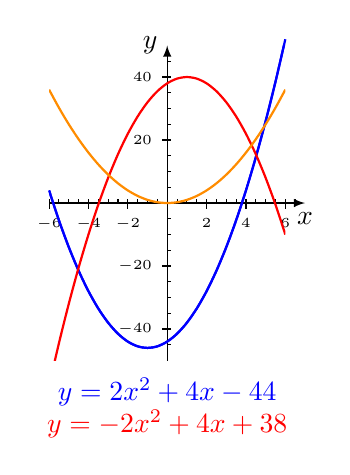
\begin{tikzpicture}[x=2.5mm,y=0.4mm,>=latex]
        \draw[thin,black,->] (-6,0) -- (7,0) node[below] {$x$};
        \draw[thin,black,->] (0,-50) -- (0,50) node[left] {$y$};
        % ticks:
        \foreach \x in {-6,-4,-2,2,4,6}
        {
          \draw[thin,black] (\x,0) -- (\x,-2pt) node[below] {$\scriptscriptstyle\x$};
        }
        \foreach \x in {-6,-5.5,...,6.5}
        {
          \draw[thin,black] (\x,0) -- (\x,1.5pt);
        }
        \foreach \y in {-40,-20,20,40}
        {
          \draw[thin,black] (0,\y) -- (-2pt,\y) node[left] {$\scriptscriptstyle\y$};
        }
        \foreach \y in {-45,-40,...,45}
        {
          \draw[thin,black] (0,\y) -- (1.5pt,\y);
        }
        \draw[thick,blue,domain=-6:6,smooth] plot (\x,{2*(\x)^2+4*\x-44});
        % graphs:
        \begin{scope}
          \clip (-6,-50) rectangle (6,50);
          \draw[thick,blue,domain=-6:6,smooth] plot (\x,{2*(\x)^2+4*\x-44});
          \draw[thick,red,domain=-6:6,smooth] plot (\x,{-2*(\x)^2+4*\x+38});
          \uncover<2->{%
            \draw[thick,orange!90!yellow,domain=-6:6,smooth] plot (\x,{(\x)^2});
          }
        \end{scope}
        % labels:
        \node[blue] at (0,-60) {$y=2x^2+4x-44$};
        \node[red] at (0,-70) {$y=-2x^2+4x+38$};
      \end{tikzpicture}
    \end{center}
  \end{minipage}
  \hfill
  \begin{minipage}{0.5\linewidth}
    \begin{itemize}
    \item $y=ax^2+bx+c$
    \item Bowl-shaped:
      \begin{itemize}
      \item[\red$\star$] Opens up if $a>0$
      \item[\red$\star$] Opens down if $a<0$
      \end{itemize}
    \item Model curve: $y=x^2$ \\
      \uncover<2->{\colorbox{blue!25}{\color{orange!90!yellow}Shown here!}}
    \end{itemize}
  \end{minipage}
  \vspace*{2in}

}

\frame{
  \frametitle{Sketching some simple graphs}


  It's useful to be able to sketch\ldots
  \smallskip

  \alert{(2)\ Cubics}

  \begin{minipage}{0.45\linewidth}
    \begin{center}
      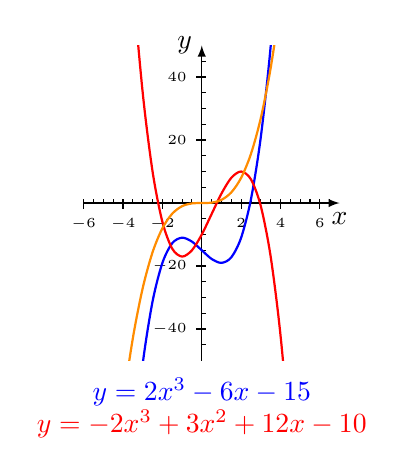
\begin{tikzpicture}[x=2.5mm,y=0.4mm,>=latex]
        \draw[thin,black,->] (-6,0) -- (7,0) node[below] {$x$};
        \draw[thin,black,->] (0,-50) -- (0,50) node[left] {$y$};
        % ticks:
        \foreach \x in {-6,-4,-2,2,4,6}
        {
          \draw[thin,black] (\x,0) -- (\x,-2pt) node[below] {$\scriptscriptstyle\x$};
        }
        \foreach \x in {-6,-5.5,...,6.5}
        {
          \draw[thin,black] (\x,0) -- (\x,1.5pt);
        }
        \foreach \y in {-40,-20,20,40}
        {
          \draw[thin,black] (0,\y) -- (-2pt,\y) node[left] {$\scriptscriptstyle\y$};
        }
        \foreach \y in {-45,-40,...,45}
        {
          \draw[thin,black] (0,\y) -- (1.5pt,\y);
        }
        % graphs:
        \begin{scope}
          \clip (-6,-50) rectangle (6,50);
          \draw[thick,blue,domain=-6:6,smooth] plot (\x,{2*(\x)^3-6*\x-15});
          \draw[thick,red,domain=-6:6,smooth] plot (\x,{-2*(\x)^3+3*(\x)^2+12*\x-10});
          \uncover<2->{%
            \draw[thick,orange!90!yellow,domain=-6:6,smooth] plot (\x,{(\x)^3});
          }
        \end{scope}
        % labels:
        \node[blue] at (0,-60) {$y=2x^3-6x-15$};
        \node[red] at (0,-70) {$y=-2x^3+3x^2+12x-10$};
      \end{tikzpicture}
    \end{center}
  \end{minipage}
  \hfill
  \begin{minipage}{0.5\linewidth}
    \begin{itemize}
    \item $y=ax^3+bx^2+cx+d$
    \item ``S''-shaped:
      \begin{itemize}
      \item[\red$\star$] Goes to $+\infty$ if $a>0$
      \item[\red$\star$] Goes to $-\infty$ if $a<0$
      \end{itemize}
    \item Model curve: $y=x^3$ \\
      \uncover<2->{\colorbox{blue!25}{\color{orange!90!yellow}Shown here!}}
    \end{itemize}
  \end{minipage}
  \smallskip
  \uncover<3->{%
    \begin{empheq}[box=\othermathbox]{align*}
      \text{For a polynomial, the {\blue highest power}\ of $x$ {\red dominates}\ when $x$ is big}    
    \end{empheq}
  }
  \vspace*{2in}



}

\section{Computing Derivatives}

\frame{
  \frametitle{The Derivatives of Simple Functions}

  \begin{minipage}{0.45\linewidth}
    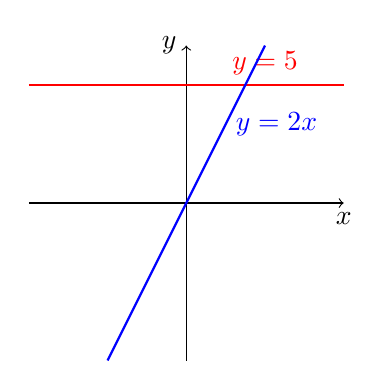
\begin{tikzpicture}
      \draw[thin,black,->] (-2,0) -- (2,0) node[below] {$x$};
      \draw[thin,black,->] (0,-2) -- (0,2) node[left] {$y$};
      \uncover<1-4>{%
        \draw[thick,red] (-2,1.5) -- (2,1.5) node[near end,above] {$y=5$};
      }
      \uncover<5->{%
        \draw[thick,blue] (-1,-2) -- (1,2) node[near end,right] {$y=2x$};
      }
    \end{tikzpicture}
  \end{minipage}
  \hfill
  \begin{minipage}{0.52\linewidth}
    The derivative of a constant is\only<1>{\ldots?}%
    \uncover<2->{%
      \ zero because:
       \begin{itemize}
       \item {\red$\text{derivative} = \text{rate of change}$}
       \item {\red constants don't change}\\[0.5em]
         \uncover<3->{%
       \item {\blue$\text{derivative} = \text{slope}$}
       \item {\blue$\text{slope} = 0$}
         }
       \end{itemize}
      \uncover<4->{So $\dfrac{d}{dx} \big( 5 \big) = 0$}
     }
  \end{minipage}
  \medskip

  \uncover<5->{%
    The derivative of a straight line is\only<5>{\ldots?}}\only<6->{%
    \ its slope because}
  \uncover<6->{%
    \begin{itemize}
    \item {\blue$\text{derivative} = \text{slope}$}
    \end{itemize}
  }
  \uncover<7->{So $\dfrac{d}{dx}\big(2x\big) = 2$}

}


\frame{
  \frametitle{Meaning of Derivatives}

  \begin{minipage}{0.45\linewidth}
    \begin{empheq}[box=\othermathbox]{align*}
      \Large%
      \frac{d}{dx}\left( x^2\right) = 2x      
    \end{empheq}
    % \vspace{.1in}

    What this {\blue means}
    %% \vspace{.1in}

    \begin{empheq}[box=\othermathbox]{align*}
      \text{The {\red slope} of the graph\ }\\
      \text{of ${\blue y=x^2}$ at $x={\red a}$ is $2{\red a}$}
    \end{empheq}
  \end{minipage}
  \hspace*{0.25in}
  \begin{minipage}{0.45\linewidth}
    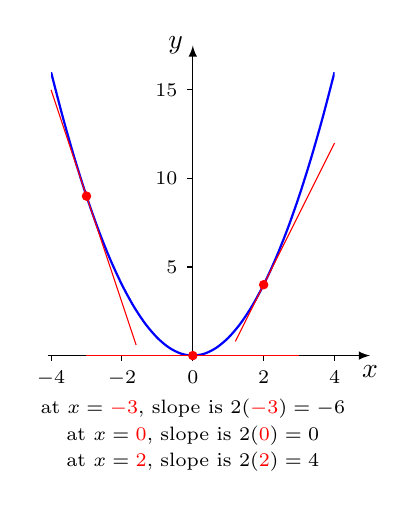
\begin{tikzpicture}[x=4.5mm,y=2.25mm,>=latex]
      \draw[thin,black,->] (-4.1,0) -- (5,0) node[below] {$x$};
      \draw[thin,black,->] (0,0) -- (0,17.5) node[left] {$y$};
      % ticks:
      \foreach \x in {-4,-2,0,2,4}
      {
        \draw[thin,black] (\x,0) -- (\x,-2pt) node[below] {$\scriptstyle\x$};
      }
      \foreach \y in {5,10,15}
      {
        \draw[thin,black] (0,\y) -- (-2pt,\y) node[left] {$\scriptstyle\y$};
      }
      \begin{scope}
        \clip (-4,0) rectangle (4,16);
        \draw[blue,thick,domain=-4:4,smooth] plot (\x,{(\x)^2});
      \end{scope}
      \uncover<2>{%
        \node at (0,-3) {$\scriptstyle\text{at $x={\red-3}$, slope is $2({\red-3})=-6$}$};
        % tangent line is y-9=-6(x+3) or y=-6x-9
        \draw[thin,red,domain=-4:-1.6] plot (\x,{-6*\x - 9});
        \filldraw[red] (-3,9) circle (1.5pt);
      };
      \uncover<3>{%
        \node at (0,-4.5) {$\scriptstyle\text{at $x={\red0}$, slope is $2({\red0})=0$}$};
        % tangent line is y=0
        \draw[thin,red] (-3,0) -- (3,0);
        \filldraw[red] (0,0) circle (1.5pt);
      };
      \uncover<4->{%
        \node at (0,-6) {$\scriptstyle\text{at $x={\red2}$, slope is $2({\red2})=4$}$};
        % tangent line is y-4=4(x-2) or y=4x-4
        \draw[thin,red,domain=1.2:4] plot (\x,{4*\x - 4});
        \filldraw[red] (2,4) circle (1.5pt);
      };
    \end{tikzpicture}
  \end{minipage}
  % \gap

  \uncover<5->{%
    \begin{empheq}[box=\othermathbox]{align*}
      \text{derivative}
      = \text{rate of change}
      = \text{slope of graph}
      = \text{slope of tangent line}
    \end{empheq}
  }



}



\frame{
  \frametitle{General Rule:}

  \begin{minipage}{0.45\linewidth}
    \begin{align*}
      \frac{d}{dx}\left(x^{\red 2}\right) & = {\red 2}x\\
      \frac{d}{dx}\left(x^{\red 3}\right) & = {\red 3}x^{\blue 2}\\
      \frac{d}{dx}\left(x^{\red 4}\right) & = {\red 4}x^{\blue 3}
    \end{align*}
  \end{minipage}
  \begin{minipage}{0.45\linewidth}
    \uncover<2->{%
      \begin{empheq}[box=\othermathbox]{align*}
        \frac{d}{dx}\left(x^{\red n}\right) & = {\red n}x^{\blue n-1}
      \end{empheq}
    }
  \end{minipage}
  \smallskip
  
  \uncover<3->{%
    The {\red exponent} comes out front. Then {\blue subtract} one
    from exponent.
  }

  \uncover<4->{\alert{Examples:}}
  \pause\pause\pause\pause

  \begin{enumerate}
  \item $\dfrac{d}{dx}\left( x^{\red 7}\right) = $
    \begin{center}
      A$ = 7x^7$
      \quad 
      B$ = 6x^6$
      \quad 
      C$ = 6x^7$
      \quad 
      D$ = 7x^6$
      \quad 
      E$ = 0$
      \quad
      \pause
      \answer{D}
    \end{center}

    \item $\dfrac{d}{dx}\left( x^{\red -3}\right) = $
      \begin{center}
        A$ = 3x^{-2}$
        \quad 
        B$ = -3x^{-2}$
        \quad 
        C$ = -2x^{-4}$
        \quad 
        D$ = -3x^{-4}$
        \quad
        \pause
        \answer{D}
      \end{center}

    \end{enumerate}

}

\frame{
  \frametitle{More Examples}
  \begin{empheq}[box=\othermathbox]{align*}
    \frac{d}{dx}\left(x^{\red n}\right) & = {\red n}x^{\blue n-1}
  \end{empheq}

  \begin{enumerate}
    \setcounter{enumi}{2}
  \item $\dfrac{d}{dx}\left( x^{\red 1/2}\right) = $
    \begin{center}
      A$ = \frac{1}{2}x^{1/2}$
      \quad 
      B$ = -\frac{1}{2}x^{-1/2}$
      \quad 
      C$ =  \frac{1}{2}x^{-1/2}$
      \quad
      \pause
      \answer{C}
    \end{center}
    \pause
  \end{enumerate}

  \alert{Rule:}\ {\red ALWAYS}\  {\blue re}write {\blue the
    thing} you want derivative of  as $x^{\red n}$
  \pause\smallskip

  \begin{enumerate}
    \setcounter{enumi}{3}
  \item $\dfrac{d}{dx}\left( {\frac{1}{x^3}}\right) = $
    \begin{center}
      A$ = \frac{1}{3x^2}$
      \quad 
      B$ = -3x^{-2}$
      \quad 
      C$ = -3x^{-4}$
      \quad
      \pause
      \answer{C}
    \end{center}
    \pause

    \item $\dfrac{d}{dx}\left({\sqrt{x}}\right) = $
      \begin{center}
        A$ =-\frac{1}{2}\sqrt{x}$
        \quad 
        B$ = \frac{1}{2}{x}^{-1/2}$
        \quad 
        C$ =  -\frac{1}{2}{x}^{-1/2}$
        \quad
        \pause
        \answer{B}
      \end{center}
  \end{enumerate}

}






\frame{
  \frametitle{Polynomials}

  \begin{equation*}
    \frac{d}{dx}\left(4x^{\red 5}+7x^{\blue 2}-{\purple 5x}+{\bluegreen 7}\right)
    = 4({\red 5})x^{\red 4}+7({\blue 2})x^{\blue 1} - {\purple 5}+{\bluegreen 0}
  \end{equation*}
  \pause

  \alert{Special cases}
  \begin{itemize}
  \item $\dfrac{d}{dx}\left( {\purple -5 x} \right)={\purple -5}$
    \pause

  \item $\dfrac{d}{dx}\left( {\bluegreen 7} \right)={\bluegreen 0}$
    \pause

  \end{itemize}
  \gap

  \begin{enumerate}
    \setcounter{enumi}{5}
  \item $\displaystyle\frac{d}{dx}\left(3x^{\red 4}+9x^{\blue 3}+{\bluegreen 7}\right)=$?
    \begin{center}
      A$ = \text{I have an answer}$
      \qquad 
      B$ = \text{I am working on it}$
      \qquad 
      C$ = \text{Help!}$
    \end{center}
  \end{enumerate}
  \pause

  \alert{Answer:}\ $12x^3+27x^2$
  \begin{center}
    A$ = \text{I got it}$
    \qquad 
    B$ = \text{I nearly got it}$
    \qquad 
    C$ = \text{I want my mommy!}$
  \end{center}


}

\section{Meaning \& Applications}

\frame{
  \frametitle{The Meanings of Derivatives}

  The derivative of $f(x)=x^2+3x+1$ is $f'(x)=\frac{df}{dx}=2x+3$.
  This means:
  \begin{itemize}
  \item[\nb] This is the {\red slope}\ of the graph $y=x^2+3x+1$ at the
    point ${\blue x}$
    \pause

  \item[\nb] It is the {\red instantaneous rate of change}\ of
    $f({\blue x})$ at ${\blue x}$.
  \pause

  \end{itemize}
  \gap

  That $f'(2) = 7$ means:
  \begin{itemize}
  \item[\nb] The {\red slope}\ of the graph $y=f({\blue x})$ at $x={\blue 2}$
    is ${\green 7}$.
    \pause

  \item[\nb] The {\red slope of the tangent line}\ to the graph at ${\blue
      x}={\blue 2}$ is ${\green 7}$.
    \pause

  \item[\nb] The {\red instantaneous rate of change}\ of $f(x)$ at
    ${\blue x}={\blue 2}$ is ${\green 7}$.
    \pause

  \item[\nb] At ${\blue x}={\blue 2}$ the output (value of $f({\blue
      x})$) changes ${\red 7}$ times as fast as the {\blue input}
    (value of ({\blue x})).
    \pause
    
  \item[\nb]  $\Delta f\approx {\red 7}\Delta {\blue x}$ near
    ${\blue x}={\blue 2}$.
    \pause

  \item[\nb] $f({\blue 2}+\Delta {\blue x})\approx f({\blue 2})+{\red 7}\Delta x$.
  \end{itemize}
 

}

\frame{
  \frametitle{Applications}

  \begin{enumerate}
    \setcounter{enumi}{6}
  \item  What is the slope of the graph $y= 3x^2-7x+5$ at $x=1$?
    \begin{center}
      A$=-2$
      \quad 
      B$=-1$
      \quad 
      C$=0$
      \quad 
      D$=1$
      \quad 
      E$=2$
      \pause
      \quad
      \answer{B}
    \end{center}
    \gap

  \item What is the instantaneous rate of change of $f(x)=x^3-2x+3$ at $x=1$?
    \begin{center}
      A$=-2$
      \quad 
      B$=-1$
      \quad 
      C$=0$
      \quad 
      D$=1$
      \quad 
      E$=2$
      \pause
      \quad
      \answer{D}
    \end{center}
    \gap

  \item After $t$ seconds a hamster on a skate board is $4t^2+2t$ cm
    from the origin on the $x$-axis. What is the exact speed of the
    hamster (in cm/sec) after $2$ seconds?
    \begin{center}
      A$=10$
      \quad 
      B$ = 16$
      \quad 
      C$ = 18$
      \quad 
      D$ = 20$
      \quad 
      E$ =14$
      \pause
      \quad
      \answer{C}
    \end{center}
  \end{enumerate}

}

\frame{
  \frametitle{Why This Works (\S8.9)}
  \begin{empheq}[box=\othermathbox]{align*}
    \frac{d}{dx}\left(x^{\red n}\right) & = {\red n}x^{\blue n-1}
  \end{empheq}

  \uncover<2->{%
    \alert{Example: $n=3$:}\ Calculate the average rate of change of
    $x^3$ between ${\blue x}$ and $x+\text{{\red\only<3->{$h$}\only<2>{$\Delta
          x$}}}$ then take limit as
    {\red\only<3->{$h$}\only<2>{$\Delta x$}}$\to 0$.
  }

  \begin{align*}
    \uncover<4->{%
    \left(
    \begin{array}{c} 
      \text{average rate}\\ 
      \text{of change between}\\ 
      \text{$x$ and $x+{\red h}$}
    \end{array}
    \right)     
    }
    & \uncover<5->{ = \frac{({ {x}+{\red h}})^{3}-{ {x}^{ 3}}}{({x}+{\red h})-{ x}}}\\
    % & = \frac{({\green x}^3+3{\green x}^2{\purple h}+3{\green x}{\purple h}^2+{\purple h}^3)-{\blue {\green x}^3}}{{\purple h}}\\ 
    % \pause
    % & = \frac{3{\green x}^2{\purple h}+3{\green x}{\purple h}^2+{\red h}^3}{{\purple h}}\\ 
    % \pause
    & \uncover<6->{= 3x^2+3x{\red h}+{\red h}^2}
  \end{align*}
  \uncover<7->{%
    Limit as ${\red h}\to0$ is \colorbox{yellow}{$3x^2$}
  }
  \gap 
  
  \uncover<8->{%
    A similar calculation works for $x^{\red n}$ for any ${\red n}$.
  }
}


\frame{
  \frametitle{More Applications}

  \begin{enumerate}
    \setcounter{enumi}{9}
  \item  What is the equation of the tangent line at $x={1}$ to the 
    graph of  $y=x^3-x+4$?  The tangent line is $y=\ldots$? 
    \begin{center}
      A$ = x+3$
      \quad 
      B$ = 3x+1$
      \quad 
      C$ = 2x-2$
      \quad 
      D$=2x+2$
      \quad 
      E$=6x-2$
    \end{center}
  \end{enumerate}
  \uncover<2->{\alert{Answer:}\ \answer{D}}

  \uncover<3->{%
    Here's a picture:

    \begin{center}
      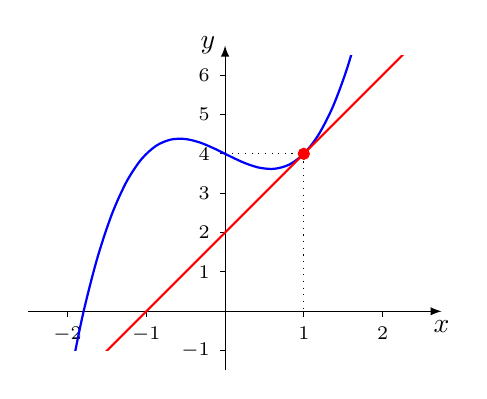
\begin{tikzpicture}[x=10mm,y=5mm,>=latex]
        \draw[thin,black,->] (-2.5,0) -- (2.75,0) node[below] {$x$};
        \draw[thin,black,->] (0,-1.5) -- (0,6.75) node[left] {$y$};
        % ticks:
        \foreach \x in {-2,-1,1,2}
        {
          \draw[thin,black] (\x,0) -- (\x,-2pt) node[below] {$\scriptstyle\x$};
        }
        \foreach \y in {-1,1,2,3,4,5,6}
        {
          \draw[thin,black] (0,\y) -- (-2pt,\y) node[left] {$\scriptstyle\y$};
        }
        \draw[thin,black,dotted] (0,4) -- (1,4) -- (1,0);
        \begin{scope}
          \clip (-2,-1) rectangle (2.5,6.5);
          \draw[thick,blue,domain=-2:2.5,smooth] plot (\x,{(\x)^3-\x+4});
        \end{scope}
        \begin{scope}
          \clip (-2,-1) rectangle (2.5,6.5);
          \draw[thick,red,domain=-2:2.5,smooth] plot (\x,{2*\x+2});
        \end{scope}
        \filldraw[red] (1,4) circle (2pt);
      \end{tikzpicture}
    \end{center}
  }
}

\frame{
  \frametitle{Another Example}

  \begin{enumerate}
    \setcounter{enumi}{10}
  \item The temperature in an oven after $t$ minutes is
    $50+t^3\ {}^{\circ}\,\text{F}$.  How quickly is the temperature
    rising after $2$ minutes?
    \begin{center}
      A$=58$
      \quad 
      B$ = 3$
      \quad 
      C$ = 12$
      \quad 
      D$ = 50$
      \quad 
      E$ = 8$
      \pause
    \end{center}
    \alert{Answer:}\ \answer{C}
  \end{enumerate}

}

\frame{
  \frametitle{A Warning!}

  \begin{empheq}[box=\othermathbox]{align*}
    \ \hfill \raisebox{-0.5em}{\dangersign[6ex]} \hspace*{0.2in}
    \frac{d}{dx}\left(f(x)g(x)\right) {\red\ne} f'(x) \times g'(x)
    \hspace*{0.2in} \raisebox{-0.5em}{\dangersign[6ex]} \hfill \ 
  \end{empheq}
  \pause
  \bigskip

  \alert{Example:} \quad 
  $5x^4
  = \dfrac{d}{dx}\left(x^5\right)
  = \dfrac{d}{dx}\left(x^2\cdot x^3\right)
  {\red\ne}(2x)(3x^2)
  =6x^3$
  \bigskip
  \pause

  \alert{Example:} Find the derivative of $(x+1)(2x+3)$
  \bigskip
  \pause

  \begin{enumerate}
    \setcounter{enumi}{11}
  \item\ $\displaystyle\frac{d}{dx}\left((x^2+1)(x^3+1)\right)=$?
    \begin{center}
      A$=6x^3$
      \quad 
      B$ = 5x^4+3x^2+2x$
      \quad 
      C$ = x^5+x^3+x^2+1$
      \quad 
      D$ = \text{Other}$
    \end{center}
    \bigskip
    \pause
  \end{enumerate}
  \alert{Answer:}\ \answer{B}

  \vspace*{2in}

}




\frame{
  \frametitle{Once upon a time\ldots} 

  There was a happy math professor and he told his
  happy students: 
  \medskip
  \pause

  ``When you work out {\blue derivatives} {\red ALWAYS} write the
  $\frac{d}{dx}$ part so you write something like
  \begin{empheq}[box=\othermathbox]{align*}
    \frac{d}{dx}\left(3x^2+5x+2\right) 
    & = 6x+5
  \end{empheq}
  and you never-ever-ever write\newline
  \begin{minipage}[b]{0.35\linewidth}
    \begin{empheq}[box=\othermathbox]{align*}
      3x^2+5x+2
      & \qquad 6x+5
    \end{empheq}
  \end{minipage}
  \hfill
  or even worse 
  \hfill
  \begin{minipage}[b]{0.35\linewidth}
    \begin{empheq}[box=\othermathbox]{align*}
      3x^2+5x+2
      =6x+5.
    \end{empheq}
  \end{minipage}
  \smallskip

  Because if you don't do as I say I will become a  sad   math professor and you will repeat this class.''

}


\end{document}

\frame{
  \frametitle{A Warning!}
  \fbox{\parbox[b]{110mm}{{\red WARNING} 
      \begin{equation*}
        \frac{d}{dx}\left(f(x)g(x)\right) {\blue\ne}\frac{df}{dx}\frac{dg}{dx}
      \end{equation*}
      \gap
      \alert{Example:} \quad $5x^4=\frac{d}{dx}\left(x^5\right)=\frac{d}{dx}\left(x^2\cdot x^3\right){\red\ne}(2x)(3x^2)=6x^3$}}
  \gap

  \alert{Example:} Find derivative of $(x+1)(2x+3)$
  \vspace*{1in}
}


\frame{
  \frametitle{An Example For You}

  \alert{Question:}\ $\displaystyle\frac{d}{dx}\left((x^2+1)(x^3+1)\right)=$?
  \begin{center}
    A$=6x^3$
    \quad 
    B$ = 5x^4+3x^2+2x$
    \quad 
    C$ = x^5+x^3+x^2+1$
    \quad 
    D$ = \text{Other}$
  \end{center}
  \bigskip
  \pause

  \alert{Answer:}\ \answer{B}

  \vspace*{2in}

}




\frame{
  \frametitle{Once upon a time\ldots} 

  There was a happy math professor and he told his
  happy students: ``When you work out {\blue derivatives} {\red ALWAYS}
  write the $\frac{d}{dx}$ part so you write something like
$$\frac{d}{dx}\left(3x^2+5x+2\right) = 6x+5$$
and you never-ever-ever write\\
\fbox{$3x^2+5x+2\qquad 6x+5$} or even worse \fbox{$3x^2+5x+2=6x+5$}

Because if you don't do as I say I will become a  sad   math professor and you will repeat this class.''

}



\frame{

$f(x)=\sqrt{x}.$ What is $f'(16) ?$\\
$A=\frac{1}{2}\quad B=\frac{1}{4}\quad C=\frac{1}{8}\quad D=\frac{1}{16}\quad E = \frac{1}{32}$\pause\quad\fbox{\blue C}\\
\ \ $\because f'(x)=\frac{1}{2}x^{-1/2}\ so\ f'(16)=\left(\frac{1}{2}\right)(16)^{-1/2}=\left(\frac{1}{2}\right)\frac{1}{\sqrt{16}}=\frac{1}{8}$

\gap
A circle is expanding so that after $R$ seconds it has radius $R$ cm.\\
What is the rate of increase of area inside the circle after 2 seconds ?\\
$A=4\pi \quad B = 2\pi R^2\quad C =2\quad D = 2\pi R\quad E = \pi R^2 $\pause\quad\fbox{\blue A}

\gap $A(R)=$ area inside circle of radius $R$\\
rate of increase of area
= derivative
= $\frac{d}{dR}\left(\pi R^2\right)=2\pi R$\\
So rate of increase of area when $R=2$ is $2\pi(2)=4\pi$

\gap What is the $x$-coordinate of the point on the graph of $y=4x^2-3x+7$ where the graph has slope ${\purple 13}$ ?\\
$A=0\quad B=1\quad C=2\quad D=3\quad E=4$\pause\quad\fbox{\blue C}

slope
= derivative\\
$=\frac{d}{dx}\left(4x^2-3x+7\right)=8x-3$\\
Want to know when this equals ${\purple 13}$\\
Solve ${\purple 13}=8x-3$ get $8x=13+3=16$ so \fbox{$x=2$}

}


\frame{


\gap
{\blue Once upon a time.....} There was a happy math professor {\red \Huge\Smiley} and he told his happy students: "When you work out {\blue derivatives} {\red ALWAYS} write the $\frac{d}{dx}$ part
so you write something like
$$\frac{d}{dx}\left(3x^2+5x+2\right) = 6x+5$$
and you never-ever-ever write\\
\fbox{$3x^2+5x+2\qquad 6x+5$} or even worse \fbox{$3x^2+5x+2=6x+5$}

Because if you don't do as I say I will become a  sad   math professor and you will repeat this class {\blue \Huge\Frowny}

}

\frame{

$f(x)=\sqrt{x}.$ What is $f'(16) ?$\\
$A=\frac{1}{2}\quad B=\frac{1}{4}\quad C=\frac{1}{8}\quad D=\frac{1}{16}\quad E = \frac{1}{32}$\pause\quad\fbox{\blue C}\\
\ \ $\because f'(x)=\frac{1}{2}x^{-1/2}\ so\ f'(16)=\left(\frac{1}{2}\right)(16)^{-1/2}=\left(\frac{1}{2}\right)\frac{1}{\sqrt{16}}=\frac{1}{8}$

\gap
A circle is expanding so that after $R$ seconds it has radius $R$ cm.\\
What is the rate of increase of area inside the circle after 2 seconds ?\\
$A=4\pi \quad B = 2\pi R^2\quad C =2\quad D = 2\pi R\quad E = \pi R^2 $\pause\quad\fbox{\blue A}

\gap $A(R)=$ area inside circle of radius $R$\\
rate of increase of area
= derivative
= $\frac{d}{dR}\left(\pi R^2\right)=2\pi R$\\
So rate of increase of area when $R=2$ is $2\pi(2)=4\pi$

\gap What is the $x$-coordinate of the point on the graph of $y=4x^2-3x+7$ where the graph has slope ${\purple 13}$ ?\\
$A=0\quad B=1\quad C=2\quad D=3\quad E=4$\pause\quad\fbox{\blue C}

slope
= derivative\\
$=\frac{d}{dx}\left(4x^2-3x+7\right)=8x-3$\\
Want to know when this equals ${\purple 13}$\\
Solve ${\purple 13}=8x-3$ get $8x=13+3=16$ so \fbox{$x=2$}

}



\frame{


\gap
{\blue Once upon a time.....} There was a happy math professor {\red \Huge\Smiley} and he told his happy students: "When you work out {\blue derivatives} {\red ALWAYS} write the $\frac{d}{dx}$ part
so you write something like
$$\frac{d}{dx}\left(3x^2+5x+2\right) = 6x+5$$
and you never-ever-ever write\\
\fbox{$3x^2+5x+2\qquad 6x+5$} or even worse \fbox{$3x^2+5x+2=6x+5$}

Because if you don't do as I say I will become a  sad   math professor and you will repeat this class {\blue \Huge\Frowny}

}

\frame{

$f(x)=\sqrt{x}.$ What is $f'(16) ?$\\
$A=\frac{1}{2}\quad B=\frac{1}{4}\quad C=\frac{1}{8}\quad D=\frac{1}{16}\quad E = \frac{1}{32}$\pause\quad\fbox{\blue C}\\
\ \ $\because f'(x)=\frac{1}{2}x^{-1/2}\ so\ f'(16)=\left(\frac{1}{2}\right)(16)^{-1/2}=\left(\frac{1}{2}\right)\frac{1}{\sqrt{16}}=\frac{1}{8}$

\gap
A circle is expanding so that after $R$ seconds it has radius $R$ cm.\\
What is the rate of increase of area inside the circle after 2 seconds ?\\
$A=4\pi \quad B = 2\pi R^2\quad C =2\quad D = 2\pi R\quad E = \pi R^2 $\pause\quad\fbox{\blue A}

\gap $A(R)=$ area inside circle of radius $R$\\
rate of increase of area
= derivative
= $\frac{d}{dR}\left(\pi R^2\right)=2\pi R$\\
So rate of increase of area when $R=2$ is $2\pi(2)=4\pi$

\gap What is the $x$-coordinate of the point on the graph of $y=4x^2-3x+7$ where the graph has slope ${\purple 13}$ ?\\
$A=0\quad B=1\quad C=2\quad D=3\quad E=4$\pause\quad\fbox{\blue C}

slope
= derivative\\
$=\frac{d}{dx}\left(4x^2-3x+7\right)=8x-3$\\
Want to know when this equals ${\purple 13}$\\
Solve ${\purple 13}=8x-3$ get $8x=13+3=16$ so \fbox{$x=2$}

}




\end{document}